\documentclass[epic,eepic,aspectratio=169,12pt]{article}
\usepackage[polish]{babel}
\usepackage[T1]{polski}
\usepackage[utf8]{inputenc}
\usepackage[T1]{fontenc}
\usepackage{color}
\usepackage{picture}
\usepackage{graphicx}
\usepackage{minibox}
\usepackage{csquotes}
%\usetheme{Copenhagen}

\usepackage[]{csquotes}
\usepackage[sorting=nty,isbn=true,backend=biber]{biblatex}

\title{Nie tylko SCRUM jest zwinny}

\author{Krzysztof Pobożan}


\begin{document}

	\maketitle
		\tableofcontents

\section{Kanban}
\subsection{Czym jest?}
	Środek do tworzenia, zarządzania i poprawy przepływo zadań dla znanej pracy.
	Pozwala organizacją w sposób płynny zmienić obecny system pracy.
	Mogą to zrobić poprzez tablicę kanbanową.
	
	Jedynym ograniczneniem jest WIP - Work In Progres ilosć zadań na raz na danym etapie pracy.
	
	Pozwala skupić się na kończeniu pracy zamiast na zaczynaniu.
\subsection{Kiedy używać?}
	\begin{itemize}
		\item Sposób wykonania zadań jest znany.
		\item Zadania napływają w sposób nie kontrolowany.
		\item Chcemy wdrażać pracę jak tylko jest gotowa, bez czekania na inne zadania.
	\end{itemize}
\subsection{Wartości}
\begin{description}
	\item[Przezroczystość] współdzielenie informacji w sposób otwarty i zrozumiały oraz ukazujący przepływ wartości biznesowej
	\item[Równowaga] różne aspekty i punkty widzenia muszą być uzwględnione aby osiągnąć efektywność
	\item[Współpraca] Jest zaprojektowany w celu polepszenia współpracy ludzi.
	\item[Koncentracja na kliencie] kanban skupia się na optymalizacji przepływu wartości dla klienta który jest z zewnątrz.

\end{description}

\section{Scrumban}

\subsection{Scrum w pigułce}
\begin{itemize}
	\item Podziel organizacje na wielo-funkcjonalne, samoorganizujące się zespoły
	\item Podziel pracę na listę małych konkretnych i dostraczalnych elementów. Posortuj listę wg. priorytetów i oszacuj względny zysk/koszt każdego elementu.
	\item Podziel czas na małe sztywne okresy (1-4 tygodnie) w trakcie których można dostarczyć coś do pokazania.
	\item Bazując na wewnętrzych spostrzeżeniach po inspekcji iteracji optymalizuj plan wdrożeń i priorytetów we współpracy z klientem.
	\item Optymalizuj proces na podstawie wniosków z retrospekcji
	\end{itemize}
\subsection{Kanban w pigułce}
\begin{itemize}
	\item Wizualizuj cykl pracy
	\begin{itemize}
		\item Podziel pracę na kawałki i umieść je na tablicy.
		\item Użyj nazw kolumn odpowiadających gdzie każdy element jest w cyklu pracy
	\end{itemize}
	\item Ogranicz WIP: przypisz limit zadań jakie mogą być na każdym etapie cyklu.
	\item Mierz czas realizacji zamówienia (średni czas) i optymalizuj w celu osiągniecia jak najmniejszego i bardziej przewidywalnego czasu.
	
\end{itemize}

\subsection{Scrumban = Scrum + Kanban}
\begin{figure}
\centering
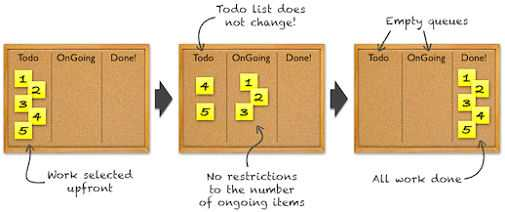
\includegraphics[width=0.7\linewidth]{what-is-scrumban-1}
\caption{Scrum}
\label{fig:what-is-scrumban-1}
\end{figure}
\begin{figure}
\centering
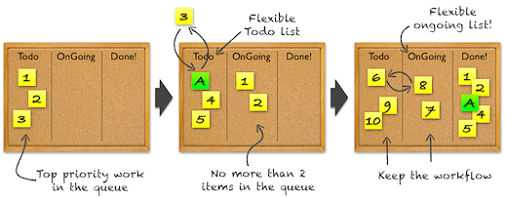
\includegraphics[width=0.7\linewidth]{what-is-scrumban-2}
\caption{Kanban}
\label{fig:what-is-scrumban-2}
\end{figure}
\begin{itemize}
	\item Używaj natury perspektywicznej ze Scruma.
	\item Używaj procesu udoskonalania z Kanbana aby pozwolić zespołowi w celu uzyskania poprawy ciągłości tego procesu.
\end{itemize}

\subsection{Zalety scrumban}
\begin{itemize}
	\item Jakoś
	\item dokładnie na czas.
	\item krótki czas
	\item Kaizen (Ciągłe polepszanie)
	\item Minimalizacja odpadków
	\item Ulepszaj proces dodając wartości ze Scruma jak potrzeba
\end{itemize}
\subsection{Kiedy stosować scrumban}
\begin{itemize}
	\item Projekty utrzymaniowe
	\begin{itemize}
		\item Praca sterowana zdarzeniami
		\item pomoc klienta/wsparcie
	\end{itemize}
	\item Mamy fazę pakowania/wydania
	\item projekt ma częste i niespodziewane US lub błędy programistyczne (niestabilny)
	\item sprinty skupione na rozwoju nowego produktu
	\item Scrum jest wyzwaniem przez cykl pracy.
\end{itemize}
\section{XP}
eXtreme Programing jest frameworkiem agile skupiającym się na wytworzniu wysokiej jakości kodu i wysokiej jakości życia zespołu programistów. Jest najbardziej specyficzny ze wszystkich technik zwinnych.
Dobre praktyki: http://ronjeffries.com/xprog/what-is-extreme-programming/
\subsection{Kiedy używać XP}

\begin{itemize}
	\item dynamicznie zmieniające się warunki oprogramowania.
	\item duże ryzyko przez limit czasowy poprzez użycie nowej technologii.
	\item zespół developerski złożony z małych grup pracujących lokalnie.
	\item technologia pozwala na pełną automatyzację testów jednosktowych i funkcjonalnych.
\end{itemize}
Więcej na http://www.extremeprogramming.org/when.html

\end{document}